

% Define a new boolean which tells us if we are compiling this as a trans
% mag paper or as part of my thesis.
\newif\iftransmagpaper

% if "\ifthesis" is defined then it's part of my thesis, otherwise it's the
% standalone paper.
\ifx\ifthesis\undefined
\transmagpapertrue
\else
\transmagpaperfalse
\fi

% \ifx\ifthesis\undefined
% \newif\ifthesis 
% \fi


% if it's the paper we need the preamble:
\iftransmagpaper

\documentclass[10pt, final, conference, transmag]{IEEEtran}

\pdfminorversion 3


%% General packages
%% ============================================================
\usepackage[cmex10]{amsmath}
\usepackage{url}                %Support for urls
\usepackage[pdftex]{graphicx}   %Needed to include pictures

\usepackage{cite} % nicer citations

\usepackage{flushend} % balance columns on last page



% Define new commands

%% Define new commands
%% ============================================================


\usepackage{amsmath}

\usepackage{xspace} % command for fixing spaces after macros


%% General Latex commands
%% ------------------------------
% New way to define commands that allows multiple subscripts
\makeatletter
\newcommand\newsubcommand[3]{\newcommand#1{#2\sc@sub{#3}}}
\def\sc@sub#1{\def\sc@thesub{#1}\@ifnextchar_{\sc@mergesubs}{_{\sc@thesub}}}
\def\sc@mergesubs_#1{_{\sc@thesub#1}}


% define a macro to allow multiple references to be passed to \cref
\newcommand\crefs[1]{\@first@ref#1,@}
\def\@throw@dot#1.#2@{#1}% discard everything after the dot
\def\@set@refname#1{%    % set \@refname to autoefname+s using \getrefbykeydefault
  \edef\@tmp{\getrefbykeydefault{#1}{anchor}{}}%
  \def\@refname{\@nameuse{\expandafter\@throw@dot\@tmp.@autorefname}s}%
}
\def\@first@ref#1,#2{%
  \ifx#2@\cref{#1}\let\@nextref\@gobble% only one ref, revert to normal \cref
  \else%
  \@set@refname{#1}%  set \@refname to autoref name
  \@refname~\ref{#1}% add autoefname and first reference
  \let\@nextref\@next@ref% push processing to \@next@ref
  \fi%
  \@nextref#2%
}
\def\@next@ref#1,#2{%
  \ifx#2@ and~\ref{#1}\let\@nextref\@gobble% at end: print and+\ref and stop
  \else, \ref{#1}% print  ,+\ref and continue
  \fi%
  \@nextref#2%
}

\makeatother

%% % The LyX greyedout annotation environment
%% \usepackage{color}
%% \definecolor{note_fontcolor}{rgb}{0.80078125, 0.80078125, 0.80078125}
%% \newenvironment{lyxgreyedout}
%% {\textcolor{note_fontcolor}\bgroup\ignorespaces}
%% {\ignorespacesafterend\egroup}

% Latin
% ============================================================

% trailing slash is needed so that latex knows the final . is not the end
% of a sentence.

\newcommand{\ie}{\textit{i.e.}\ }
\newcommand{\cf}{\textit{c.f.}\ }
\newcommand{\eg}{\textit{e.g.}\ }
\newcommand{\etal}{\textit{et al.}\ }
\newcommand{\etc}{etc.\ }



%% General maths commands
%% ------------------------------
\newcommand{\pd}[2]{\frac{\partial #1}{\partial #2}} % partial deriv
\newcommand{\spd}[2]{\frac{\partial^2 #1}{\partial {#2}^2}} % 2nd partial deriv
\newcommand{\ddn}[1]{\pd{#1}{\nv}} % normal derivative
\newcommand{\variation}{\delta}
\newcommand{\vd}[2]{\frac{\variation #1}{\variation #2}} % variational derivative
\newcommand{\myvector}[1]{\boldsymbol{\mathrm{#1}}}
\newcommand{\goesto}{\rightarrow}
\newcommand{\mean}{\operatorname{mean}}

% Write paragraphs in an equation environment with nice spacing, line wraps
% etc. eg for fem problem statements.
\newcommand{\eqpar}[1]{\text{\parbox{0.8\textwidth}{#1}}}

\newcommand{\set}[1]{\left\{ {#1} \right\}}
\newcommand{\setst}[2]{\left\{ {#1} \,\middle|\, {#2} \right\}}

\newcommand{\E}[1]{\times 10^{#1}} % powers of 10
\newcommand{\st}{\,|\,} % ``such that'' operator in sets (vertical line with spacing)

\newcommand{\ip}[2]{\left(#1,\, #2 \right)} % inner product
\newcommand{\ltip}[2]{\ip{#1}{#2}_{\ltwo}} % l2 inner product


% Norm and abs
\newcommand{\abs}[1]{\left|{#1} \right|}
% \newcommand{\norm}[1]{\lVert #1 \rVert}
\newcommand{\norm}[1]{\left| \left| #1 \right| \right|}
\newcommand{\ltnorm}[1]{\norm{#1}_{\ltwo}}
\newcommand{\determinant}[1]{\left|{#1} \right|}


% rescaled time
\newcommand{\that}{\hat{t}}

% d for the end of integrals (e.g. dx) with correct spacing and non-italic.
\renewcommand{\d}{{\; \mathrm{{d}}}}

% standard integrals
\newcommand{\intd}[2][\magd]{{\int_{#1} {#2} \d {#1}}}
\newcommand{\intdx}[2][\magd]{{\int_{#1} {#2} \d \xv}}
\newcommand{\intds}[2][\magd]{{\int_{#1} {#2} \d \sv}}

\newcommand{\intb}[1]{\intd[\boundd]{#1}}
\newcommand{\intui}[2][x]{{\int_0^1 #2 \d{#1}}} % unit interval

\newcommand{\intt}[1]{{\int_T {#1} \d t}}


% Jacobian of transformation
\newcommand{\jstox}{J}

% Some vector functions
\newcommand{\gv}{{\myvector{g}}}
\newcommand{\fv}{{\myvector{f}}}
\newcommand{\pv}{{\myvector{p}}}


\newcommand{\ffv}[1]{{\myvector{f}\bigb{#1}}}
\newcommand{\gfv}[1]{{\myvector{g}\bigb{#1}}}


% Some vectors
\newcommand{\av}{{\myvector{a}}}
\newcommand{\bv}{{\myvector{b}}}
\newcommand{\cv}{{\myvector{c}}}
\newcommand{\sv}{{\myvector{s}}}
\newcommand{\kvec}{\myvector{k}}
\newcommand{\vv}{{\myvector{v}}}

\newcommand{\ev}{\myvector{\hat{e}}}
\newcommand{\nv}{\myvector{\hat{n}}}

\newcommand{\xv}{\myvector{x}}
\newcommand{\yv}{\myvector{y}}
\newcommand{\wv}{\myvector{w}}
\newcommand{\dydt}{\pd{\yv}{t}}
\newcommand{\zv}{\myvector{z}}
\newcommand{\lv}{\myvector{l}}

\newcommand{\unitv}[1]{{\hat{\mathbf{#1}}}}
\newcommand{\iv}{\unitv{i}}
\newcommand{\jv}{\unitv{j}}
\newcommand{\kv}{\unitv{k}}
\newcommand{\unitz}{\unitv{z}}

% Matrices
\newcommand{\mymatrix}[1]{\mathrm{#1}}
\newcommand{\mat}{\Bm}

\newcommand{\Pm}{\mymatrix{P}}
\newcommand{\Qm}{\mymatrix{Q}}
\newcommand{\Idm}{\mymatrix{I}}
\newcommand{\Am}{\mymatrix{A}}
\newcommand{\Gm}{\mymatrix{G}}
\newcommand{\Fm}{\mymatrix{F}}
\newcommand{\Mm}{\mymatrix{M}}
\newcommand{\Jm}{\mymatrix{J}}
\newcommand{\Km}{\mymatrix{K}}
\newsubcommand{\Jmca}{\mymatrix{J}}{\mathrm{ca}}
\newcommand{\Jmts}{J_\mathrm{ts}}

\newcommand{\Bm}{\mymatrix{B}}
\newcommand{\Cm}{\mymatrix{C}}
\newcommand{\Dm}{\mymatrix{D}}

% Preconditioners
\newcommand{\precond}{\mathcal{P}}
\newcommand{\preca}{\precond_1}
\newcommand{\precb}{\precond_2}
\newcommand{\precc}{\precond_3}

\newcommand{\inexact}[1]{\widetilde{#1}}
\newcommand{\parinexact}[1]{\bar{#1}}
\newcommand{\pbin}{\inexact{\precb}}
\newcommand{\pcin}{\inexact{\precc}}


% Make ams math matrices allow dividing lines
\makeatletter
\renewcommand*\env@matrix[1][*\c@MaxMatrixCols c]{%
  \hskip -\arraycolsep
  \let\@ifnextchar\new@ifnextchar
  \array{#1}}
\makeatother


% constants in front of Jacobian
\newcommand{\cts}{c_\mathrm{ts}}
\newcommand{\jts}{\frac{\cts}{\dtn}}

% Brackets
\newcommand{\bigb}[1]{{\left( #1 \right)}}
\newcommand{\bigs}[1]{{\left[ #1 \right]}}
\newcommand{\evalat}[1]{{\left|_{#1}\right.}}
\newcommand{\evalatb}[2]{{\left. {#1} \right|_{#2}}}


% BEM
\newcommand{\bm}{{\mathbf{\Gm}}}
\newcommand{\tri}{\vartriangle}



% 3-component vector as a list of components
\newcommand{\threevec}[3]{\begin{pmatrix} #1 \\ #2 \\ #3 \end{pmatrix} }
\newcommand{\threevecdup}[1]{\threevec{#1}{#1}{#1}}
\newcommand{\threevecnum}[1]{\threevec{#1_0}{#1_1}{#1_2}}


% Big O notation
\newcommand{\order}[1]{\mathrm{O}\bigb{#1}}

% Differential operators
\renewcommand{\div}{\nabla \cdot} % \div is normally division
\newcommand{\grad}{\nabla}
\newcommand{\curl}{\nabla \times}
\newcommand{\lap}{\nabla^2}
\newcommand{\disclap}{\widetilde{\Delta}}


% grad of a vector
\newcommand{\gradv}{\widetilde{\grad}}


\newcommand{\compdot}{\mathbin{:}}
\newcommand{\tensorprod}{\otimes}



%% Spaces, domains and geometrical labels
%% ------------------------------
% Domain labels used
\newcommand{\magd}{\Omega}
\newcommand{\boundd}{{\Gamma}}
\newcommand{\fulld}{{\real^d}}
\newcommand{\extd}{{\Omega^c}}

% Interior/exterior labels
\newcommand{\inte}{\mathrm{int}}
\newcommand{\exte}{\mathrm{ext}}

\newcommand{\real}{\mathbb{R}} % real numbers
\newcommand{\complex}{\mathbb{C}} % complex numbers
\newcommand{\integers}{\mathbb{Z}} % integer numbers

\newcommand{\sob}{\mathcal{H}} % Sobelov spaces
\newcommand{\ltwo}{{L^2}} %L2

\newcommand{\Neu}{{\scriptscriptstyle{\mathcal{N}}}} % Neumann
\newcommand{\Dir}{{\scriptscriptstyle{\mathcal{D}}}} % Neumann

\newcommand{\Htest}{\sob^1_0(\magd)}
\newcommand{\Hsol}{\sob^1_D(\magd)}

\newcommand{\krylov}{\mathcal{K}}
\DeclareMathOperator{\spanop}{span}



%% Magnetics
%% ------------------------------
% Define M, H, B vectors (i.e. bold)
\newcommand{\Mv}{\myvector{M}}
\newcommand{\Hv}{\myvector{H}}
\newcommand{\Bv}{\myvector{B}}


% polar coords
\newcommand{\ruv}{\myvector{\hat{r}}} % r unit vector
\newcommand{\phiv}{\myvector{\hat{\phi}}}
\newcommand{\thetav}{\myvector{\hat{\theta}}}
\newcommand{\rv}{\myvector{r}} % r vector


% Define some common types of H-field.
% if changing these beware of components of H which are not defined here.
\newsubcommand{\Heff}{\myvector{H}}{{\mathrm{eff}}} %effective (total)
\newsubcommand{\Happ}{\myvector{H}}{{\mathrm{ap}}} %applied
\newsubcommand{\Hms}{\myvector{H}}{\mathrm{ms}} % magnetostatic/demag
\newsubcommand{\Hex}{\myvector{H}}{\mathrm{ex}} % exchange
\newsubcommand{\Hca}{\myvector{H}}{\mathrm{ca}} % crystalline ansiotropy
\newsubcommand{\Hthm}{\myvector{H}}{\mathrm{th}} % thermal

\newcommand{\phim}{\phi} % magnetostatic potential
\newcommand{\phione}{u} % auxilary potential
\newcommand{\phitwo}{v} % other auxilary potential

% Normalised versions of the above fields (and M)
\newcommand{\mv}{\myvector{m}}
\newcommand{\hv}{\myvector{h}}
\newsubcommand{\heff}{\myvector{h}}{{\mathrm{eff}}} %effective (total)
\newsubcommand{\happ}{\myvector{h}}{{\mathrm{ap}}} %applied
\newsubcommand{\hms}{\myvector{h}}{\mathrm{ms}} % magnetostatic/demag
\newsubcommand{\hex}{\myvector{h}}{\mathrm{ex}} % exchange
\newsubcommand{\hca}{\myvector{h}}{\mathrm{ca}} % crystalline ansiotropy
\newsubcommand{\hthm}{\myvector{h}}{\mathrm{th}} % thermal
\newcommand{\nH}{H_{\mathbb{n}}} % A "magnitude" of H for normalisation

% Similarly for energies
\newsubcommand{\Eapp}{E}{{\mathrm{ap}}} %applied
\newsubcommand{\Ems}{E}{\mathrm{ms}} % magnetostatic/demag
\newsubcommand{\Eex}{E}{\mathrm{ex}} % exchange
\newsubcommand{\Eca}{E}{\mathrm{ca}} % crystalline ansiotropy
\newcommand{\e}{e} % total energy
\newsubcommand{\eapp}{\e}{{\mathrm{ap}}} %applied
\newsubcommand{\ems}{\e}{\mathrm{ms}} % magnetostatic/demag
\newsubcommand{\eex}{\e}{\mathrm{ex}} % exchange
\newsubcommand{\eca}{\e}{\mathrm{ca}} % crystalline ansiotropy
\newsubcommand{\ehop}{\e}{\hop} % total due to h operator fields


\newcommand{\nE}{E_{\mathbb{n}}} % A "magnitude" of energy for normalisation
\newcommand{\nA}{\mathbb{A}} % A "magnitude" of exchange const for normalisation
\newcommand{\nK}{\mathbb{K}} % A "magnitude" of anisotropy const for normalisation

% Magnetic constants
\newcommand{\Exchc}{A}
\newcommand{\Kone}{K_1}
\newcommand{\kone}{\mathcal{K}_1}
\newcommand{\dampc}{\alpha}
\newcommand{\dampeff}{\alpha_\mathrm{eff}}
\newcommand{\gymagc}{{\abs{\gamma_{\mathrm{\tiny{L}}}}}}
\newcommand{\scc}{\beta} % The constant in front of the self-correcting LLG
                         % term


% SI magnetic units
\newcommand{\Mu}{{\mathrm{Am}^{-1}}}
\newcommand{\Hu}{{\mathrm{Am}^{-1}}}
\newcommand{\phiu}{{\mathrm{A}}} % magnetic potentials
\newcommand{\Bu}{{\mathrm{T}}}
\newcommand{\gymagu}{{\mathrm{A}(\mathrm{ms})^{-1}}}

% Define the LLG equation (in parts then all together)
\newcommand{\dMdt}{\pd{\Mv}{t}} % define dM/dt
\newcommand{\dmdt}{\pd{\mv}{t}}
\newcommand{\dMdn}{\pd{\Mv}{\nv}}
\newcommand{\dmdn}{\pd{\mv}{\nv}}

\newcommand{\MxH}{\Mv \times \Hv} % define M x H
\newcommand{\mxh}{\mv \times \hv}
\newcommand{\mxmxh}{\mv \times \bigb{\mv \times \hv}}
\newcommand{\MxdMdt}{\Mv \times \dMdt}
\newcommand{\mxdmdt}{\mv \times \dmdt}
\newcommand{\llg}{\dmdt = -(\mxh) + \dampc (\mxdmdt)}

%% Finite elements/numerical models
%% ------------------------------
% Define the test and shape functions
\newcommand{\tbf}{\varphi}
\newcommand{\tbfv}{\myvector{\varphi}}
\newcommand{\test}{v}
\newcommand{\testv}{\myvector{\test}}

\newcommand{\sumbasiscoeff}{C}

\newcommand{\sbf}{\psi}
\newcommand{\ts}{{\sob^1_h(\magd)}} % my test/shape fn space
\newcommand{\tsinf}{{\sob^1(\magd)}} % my infinite test/shape fn space
\newcommand{\tsbasis}[1][{}]{{S^1_{#1}(\magd)}} % test/shape basis functions

\newcommand{\sk}{{\sbf_k}}
\newcommand{\tn}{{\tbf_\ndi}}

% Indices
\newcommand{\ndi}{n} % nodal index, not sure what to have it as...
\newcommand{\eli}{e} % element index
\newcommand{\tl}{l} % time-step index

% Green's functions - general form and main parts of 2/3D Green's functions for the laplacian operator
\newcommand{\Green}[1][]{G(\xv_{#1},\yv)}
\newcommand{\Gtwod}[1][]{\ln \abs{\xv_{#1} - \yv}}
\newcommand{\Gthreed}[1][]{\frac{1}{ \abs{\xv_{#1} - \yv}}}

% subscripts used
\newcommand{\ibasis}{{i}}
\newcommand{\ibasisb}{{j}}
\newcommand{\ibasisc}{{k}}

% Write some names nicely
\newcommand{\mumag}{\textmu{}mag\xspace}
\newcommand{\oomph}{\texttt{oomph-lib}\xspace}
\newcommand{\nmag}{Nmag\xspace}
\newcommand{\magpar}{magpar\xspace}
\newcommand{\femme}{femme\xspace}
\newcommand{\oommf}{OOMMF\xspace}
\newcommand{\vode}{VODE\xspace}
\newcommand{\cvode}{CVODE\xspace}

\newcommand{\hypre}{Hypre\xspace}
\newcommand{\superlu}{SuperLU\xspace}
\newcommand{\hlib}{HLib\xspace}


%% Time stepping
%% ------------------------------

% time step
\newcommand{\dtn}{\dtx{n}}
\newcommand{\dtx}[1]{\Delta_{#1}}

% "value step"
% Getting bold greek requires a hack because mathbf sees it as a "symbol"
% and so doesn't change it. This uses the direct TeX solution (from google!)
\newcommand{\dyn}{\dyx{n}}
\newcommand{\dyx}[1]{\mbox{\boldmath$\delta$}_{#1}}

% Denote various time steppers
\newcommand{\AB}{\mathrm{AB}} % Adams-Bashforth 2
\newcommand{\imr}{\mathrm{IMR}} % Implicit midpoint
\newcommand{\tr}{\mathrm{TR}}
\newcommand{\bdf}{\mathrm{BDF2}}
\newcommand{\bdfo}{\mathrm{BDF1}}
\newcommand{\FE}{\mathrm{FE}} % Forward Euler (like)
\newcommand{\ebdf}{\mathrm{eBDF3}}

% Local truncation errors
\newcommand{\lte}{T_n}

% Tol
\newcommand{\toltt}{\epsilon_{\dtx{}}}
\newcommand{\mltol}{\epsilon_{\mathrm{ml}}}


% Newton's method
% ============================================================

% tol
\newcommand{\newtontol}{\epsilon_{\mathrm{N}}}
\newcommand{\ntol}{\newtontol}
\newcommand{\nrtol}{\epsilon_{\mathrm{Nr}}}


% list of discrete values
\newcommand{\mydiscrete}[1]{\tilde{#1}}
\newcommand{\mvdis}{\mydiscrete{\mv}}
\newcommand{\yvdis}{\mydiscrete{\yv}}
\newcommand{\wvdis}{\mydiscrete{\wv}}
\newcommand{\phionedis}{\mydiscrete{\phione}}
\newcommand{\phimdis}{\mydiscrete{\phim}}


% approximation functions (fem)
\newcommand{\myinterp}[1]{{#1}_h}
\newsubcommand{\mvh}{\mv}{h}
\newcommand{\phimh}{\myinterp{\phim}}
\newcommand{\dmdth}{\pd{\mvh}{t}}
\newcommand{\testh}{\myinterp{\test}}
\newcommand{\testvh}{\myinterp{\testv}}



\newcommand{\resi}{\rv}
\newcommand{\jac}{\mathrm{J}}
\newcommand{\nlit}[2]{{#1}^{(#2)}}
\newcommand{\nowy}{\nlit{\yvdis}{0}}
\newcommand{\nexty}{\yvdis^E}
\newcommand{\corr}{\myvector{\delta}}

% Operators
% ============================================================
\usepackage{mathrsfs}
\newcommand{\myop}[1]{\mathscr{#1}}
\newcommand{\hop}{\myop{H}}
\newcommand{\hopb}[1]{\myop{H} \bigs{#1}}

\newcommand{\hmsop}{\myop{H}_{\mathrm{ms}}}
\newcommand{\aop}{\myop{A}}
\newcommand{\bop}{\myop{B}}
\newcommand{\cop}{\myop{C}}
\newcommand{\lop}{\myop{L}}
\DeclareMathOperator{\realp}{Re}

% Fractions
% ============================================================

%% Nice one line fractions
\usepackage{xfrac}
\usepackage[ugly]{nicefrac}

\newcommand{\half}{\nicefrac{1}{2}}



% Stuff needed for galerkin
% ============================================================
\newcommand{\skewop}{\text{\Large{$\Lambda$}}}
\newcommand{\skewm}[1]{\skewop\left[ #1 \right]}
\newcommand{\crossop}[2]{\skewm{ #1 } \cdot \left( #2 \right)}

\newcommand*\circled[1]{\tikz[baseline=(char.base)]{
    \node[shape=circle,draw,inner sep=1pt] (char) {#1};}}
\newcommand{\mxex}{I}
\newcommand{\mxmxex}{J}

\newcommand{\intp}[1]{\sum_\ibasisc \sk #1_\ibasisc}
\newcommand{\intpb}[1]{\left( \intp{#1} \right)}
\newsubcommand{\hs}{\hv}{\mathrm{s}}

\newcommand{\ik}{\ibasisc}

% residuals
\newsubcommand{\rex}{\myvector{r}}{\mathrm{ex}}
\newsubcommand{\rexh}{\myvector{r}}{\mathrm{ex,h}}
\newsubcommand{\rll}{\myvector{r}}{\mathrm{ll}}
\newcommand{\rllg}{r}
\newcommand{\rllgv}{\myvector{\rllg}}
\newcommand{\rphi}{s}

% strong form residuals
\newcommand{\Rllg}{\myvector{\mathcal{R}}}
\newcommand{\Rphi}{\mathcal{S}}



% Notation for midpoint method stuff
% ============================================================

% t at midpoint
\newcommand{\thfx}[1]{t_{#1+\half}}
\newcommand{\thf}{\thfx{n}}

% exact y of t at midpoint
\newcommand{\yvhfx}[2]{\yv#1(\thfx{#2})}
\newcommand{\yvhf}[1][]{\yvhfx{#1}{n}}

% midpoint approximation to y
\newcommand{\yvmx}[1]{\yv_{#1+\half}}
\newcommand{\yvm}{\yvmx{n}}


% df/dy matrix
\newcommand{\dfdy}{F}
\newcommand{\dfdyhfx}[1]{\dfdy_{#1+\half}}
\newcommand{\dfdyhf}{\dfdyhfx{n}}

% error due to midpoint approx
\newcommand{\ymiderr}{a_n}

% full expressions for midpoint values
\newcommand{\mpm}{\frac{\mv_{n+1} + \mv_n}{2}}
\newcommand{\mpt}{\frac{t_n + t_{n+1}}{2}}
\newcommand{\mpdmdt}{\frac{\mv_{n+1} - \mv_n}{\dtn}}
\newcommand{\mphop}{\hop \left[ \mpm \right]}
\newcommand{\mphapp}{\happ \left(\mpt \right)}

% temp bdf1 values
\newcommand{\midp}{{\mathrm{mid}}}



% Commands from intermag paper
% ============================================================

\newcommand{\dash}{\mathrm{-}}
\newcommand{\dtinitial}{\dtx{\mathrm{init}}}
\newcommand{\dtmax}{\dtx{\mathrm{max}}}
\newcommand{\zerov}{\mathbf{0}}
\newcommand{\mvtemp}{\mv_*}



% Error norms
% ============================================================

\newcommand{\myerr}{\mathcal{E}}

% switching time error
\newsubcommand{\swtimeerr}{\myerr}{\tau}

% ode m error
\newsubcommand{\merr}{\myerr}{\mv}

% pde m error, captions hate \newsubcommand for some reason so just use
% newcommand
\newcommand{\errmpde}{\myerr{}_{\mv}}

\newcommand{\errphase}{\myerr_p}
\newcommand{\errmz}{\myerr_{m_z}}

\newcommand{\errml}{\myerr_{\abs{\mv}}}



% Numbers of things
% ============================================================
\newcommand{\nrow}{N_r} % matrix rows
\newcommand{\Nn}{N} % nnodes
\newcommand{\Nb}{N_\boundd} % boundary nodes
\newcommand{\Nbul}{N_\magd} % bulk nodes

%%% Local Variables:
%%% mode: latex
%%% TeX-master: "main"
%%% End:


% custom commands for transmag standards
\renewcommand{\figpos}{t!}
\newcommand{\figsize}{3.5in}

\def\figureautorefname{Fig.}



\title{Discretisation induced stiffness in micromagnetic simulations}

\newcommand{\uom}{The University of Manchester, Oxford Road, Manchester, M13 9PL, UK}

\author{\IEEEauthorblockN{David Shepherd\IEEEauthorrefmark{1},
    Jim Miles\IEEEauthorrefmark{1},
    Matthias Heil\IEEEauthorrefmark{2},
    Milan Mihajlovi\'{c}\IEEEauthorrefmark{1}}
  \IEEEauthorblockA{\IEEEauthorrefmark{1} School of Computer Science, \uom{}} 
  \IEEEauthorblockA{\IEEEauthorrefmark{2} School of Mathematics, \uom{}}%
}


\begin{document}

\IEEEtitleabstractindextext{%
  \begin{abstract}
    In the numerical integration of the Landau-Lifshitz-Gilbert (LLG) equation, stiffness (stability restrictions on the time step size for explicit methods) is known to be a problem in some cases.  
    We examine the relationship between stiffness and spatial discretisation size for the LLG with exchange and magnetostatic effective fields.
    A maximum stable time step is found for the reversal of a single domain spherical nanoparticle with a variety of magnetic parameters and numerical methods.
    From the lack of stiffness when solving a physically equivalent ODE problem we conclude that any stability restrictions in the PDE case arise from the spatial discretisation rather than the underlying physics.

    We find that the discretisation induced stiffness increases as the mesh is refined and as the damping parameter is decreased.
    In addition we find that use of the FEM/BEM method for magnetostatic calculations increases the stiffness.
    Finally, we observe that the use of explicit magnetostatic calculations within an otherwise implicit time integration scheme (\ie a semi-implicit scheme) does not cause stability issues.
  \end{abstract}
  \begin{IEEEkeywords}
    Numerical stability, Micromagnetics
  \end{IEEEkeywords}}


\maketitle

\IEEEdisplaynontitleabstractindextext


% otherwise we need the chapter title (and some commands are modified)
\else
\chapter{Stiffness of the LLG equation}
\label{cha:stiffn-llg-equat}


\newcommand{\fig}{Figure~}
\newcommand{\figs}{Figures.~}
\newcommand{\figsize}{0.6\textwidth}


\fi

% Now start the writing for real!

\section{Introduction}

Dynamic micromagnetic simulations  center around solving the Landau-Lifshitz-Gilbert (LLG) equation with various effective fields.
In this paper we focus on continuum mechanics models of micromagnetics, where the LLG with exchange becomes a system of partial differential equations (PDEs).
For such models stiffness (the restriction of time step size by stability rather than by the desired accuracy) has long been recognised as an issue, at least for some problems
\cite{Nakatani1989}.

Stiffness in PDEs has at least two possible sources: 
firstly a problem may be physically stiff due to large differences in the characteristic time scales of different (physical) components of the solution \cite[Chap. 4]{Iserles2009};
secondly the choice of spatial discretisation method may cause stiffness.
In particular a fine spatial discretisation often results in a stiff system of ODEs.
An intuitive explanation for this is that a finer mesh resolves shorter wavelength modes, even if they have almost no effect on the resulting solution.
Shorter wavelength implies higher frequency, \ie shorter characteristic time scales.
These modes interact with the solution, and the large variation in time scales causes stiffness in a similar way to physical effects.
For a rigorous discussion of this effect in terms of the eigenvalues of the time integration operator see e.g. \cite[Sec 8.2]{Atkinson2009}.

\iftransmagpaper Time  \else As discussed in \autoref{sec:time-discretisation} time \fi integration methods can be roughly divided into two classes: those which are not good at solving stiff problems and those which are.
These two classes correspond to \emph{explicit} methods that calculate the value at the next time exclusively in terms of previous values and \emph{implicit} methods in which a system of equations must be solved. 
Typically one step of an implicit method requires more computational effort than a step of an explicit method because of this solve.
However good implicit methods are unconditionally stable, allowing them to take much larger time steps when applied to stiff problems \cite[Chap. 4]{Iserles2009}.
Hence there is a trade-off between time step size and the computational effort per step.
Since the optimal choice depends on the stiffness it is important to understand its origins in micromagnetic simulations.

In this \iftransmagpaper paper \else chapter \fi we examine numerically the relationship between stiffness and spatial discretisation size for a simple micromagnetic problem where stiffness due to physical effects can be ruled out.
We also explore how stiffness is affected by the use of the FEM/BEM method for magnetostatic calculations.
Finally, we study the effects of stiffness on methods which combine explicit magnetostatic calculations with implicit exchange field and LLG calculations (\ie semi-implicit methods).

\section{The model}

\iftransmagpaper
We compute the time dependent behaviour of magnetisation, $\mv = \mv(\xv, t)$, using the non-dimensionalised
Landau-Lifshitz-Gilbert equation \cite{Aharoni1996} with dimensionless Gilbert damping constant $\dampc$
\begin{equation}
  \begin{aligned}
    \dmdt &= - \mv \times \hv + \dampc \mv \times \dmdt, \\
    \hv &= \lap \mv + \hms + \happ. \label{llg}
  \end{aligned}
\end{equation}
Here $\hms$ is the magnetostatic field and $\happ$ is the applied field, both in units of the saturation magnetisation, $M_s$.
Unit distance is the magnetostatic exchange length,
$\sqrt{\frac{2A}{\mu_0 M_s^2}} \approx 1\text{-}10\text{nm}$.
Unit time is $(|\gamma| M_s)^{-1} \approx 5\text{ps}$.
Standard boundary conditions for zero surface anisotropy are used, \ie $\pd{\mv}{\nv} = \mathbf{0}$ where $\nv$ is the outer unit normal.

The magnetostatic field is calculated via a scalar potential
using the FEM/BEM method \cite{Fredkin1990}\cite{Knittel2011}
\begin{equation}
  \begin{aligned}
    \label{eq:fem-bem}
    \lap \phione = \nabla \cdot \mv, \\
    \lap \phim = \nabla \cdot \mv, \\
    \hms = -\grad \phim,
  \end{aligned}
\end{equation}
where $\phim$ is the standard magnetostatic potential and $\phione$ is an auxiliary potential used to apply the boundary condition $\lim_{|\xv| \rightarrow \infty} \phim = 0$.
The corresponding boundary conditions are $\pd{\phione^\inte}{\nv} = \mv \cdot \nv$ and $\phim = \bm \big[ \phione \big]$, where $\bm$ is the BEM operator. After discretisation by collocation the BEM operator is a dense matrix with elements given by
\begin{equation}
  \begin{aligned}
    \bm_{ij} = \frac{\gamma(\xv_i)\delta_{ij}}{4\pi} 
- \frac{1}{4 \pi} \int_\boundd \varphi_{j}(\yv) \frac{\nv(\yv) \cdot (\yv - \xv_{i} )}{\abs{\yv - \xv_i} ^2} \d \yv,
    \label{eq:bem-matrix}
  \end{aligned}
\end{equation}
where $\boundd$ is the boundary of the magnetic region, $\xv_i$ is the location of node $i$, $\varphi_{i}$ is the corresponding shape function and $\gamma(\xv_i)$ is the solid angle filled by the magnetic region as $ \xv \rightarrow \xv_i$.
The singular integrals in \eqref{eq:bem-matrix} can be evaluated analytically for linear triangular elements using the Lindholm formula\cite{Lindholm1984}.
The boundary value of $\phim$ at node $j$ is given in terms of \emph{all} the boundary values of $\phione$ by $\phim_j = \sum_i \bm_{ij} \phione_i$ (\ie by a dense matrix multiplication on the vector of nodal values).
Details and a derivation of the FEM/BEM method may be found in \cite[Sec 2.2]{Knittel2011}.

% It should be noted that FEM/BEM models more commonly solve for $\phione$ and $\phi_2$ then use $\phim = \phione + \phi_2$. We prefer to calculate $\phim$ directly because it simplifies some implementation issues. The two approaches are mathematically equivalent.

For all equations other than the BEM operator a standard linear Galerkin finite
element discretisation is used \cite[25]{HowardElmanDavidSilvester2006}.
\else
In these experiments we use the FEM discretisation of the non-dimensionalised LLG as discussed in \autoref{sec:galerk-meth-llg}.
When in use magnetostatics are handled using the FEM/BEM discretisation as discussed in \autoref{sec:hybr-finit-elem}.
\fi

\subsection{Implicit time integration}
For implicit integration we use the implicit midpoint rule (IMR)
\iftransmagpaper
\cite{dAquino2005}
\begin{equation}
  \label{eq:imr}
  \begin{aligned}
    \mv_{n+1} = \mv_n + \dtn 
    f\left(
      \frac{t_{n+1} + t_n}{2}, \frac{\mv_{n+1} + \mv_n}{2}
    \right),
  \end{aligned}
\end{equation}
where $f(t, \mv) = \pd{\mv}{t}(t, \mv)$ and $\dtn = t_{n+1} - t_n$.
\else
with constant time steps as discussed in \autoref{sec:adaptive-imr}.
\fi
The complete problem (including the magnetostatic potential equations) is then linearised using Newton's method.
The resulting linear system is solved using GMRES with an incomplete LU decomposition\footnote{Hypre's Euclid preconditioner\cite{hypre} with no drop tolerance and factorisation level 1.} of the sparse parts of the system as a preconditioner, ignoring the dense block in the Jacobian arising from \iftransmagpaper\eqref{eq:bem-matrix}\else the BEM\fi.

\subsection{Explicit time integration}
For the explicit integration we need to use an explicit rearrangement \cite[181]{Aharoni1996} of \iftransmagpaper\eqref{llg}\else the LLG equation\fi
\begin{equation}
  \label{eq:ll}
  \begin{aligned}
    \dmdt (1 + \dampc^2) &= - \mv \times \hv - \dampc \mv \times \left( \mv \times \hv \right).
  \end{aligned}
\end{equation}
As the time integrator we use a two stage Runge-Kutta method (RK2), also known as Heun's method:
\begin{equation}
  \label{eq:heunn}
  \begin{aligned}
    \mvtemp &= \mv_n + \dtn f(t_n, \mv_n), \\
    \mv_{n+1} &= \mv_n + \frac{\dtn}{2} \left( f(t_n, \mv_n) + f(t_{n+1},
      \mvtemp) \right).
  \end{aligned} 
\end{equation}
Time derivatives are calculated within the Galerkin method by inverting the finite-element mass matrix using a diagonally preconditioned conjugate gradient solver.
The magnetostatic potential $\phim$ is recalculated using the FEM/BEM method at appropriate time and magnetisation values during each stage of \eqref{eq:heunn}.
The Poisson solves\iftransmagpaper, \eqref{eq:fem-bem},\fi{} required for the evaluation of the potentials $\phione$ and $\phim$ use a conjugate gradient solver preconditioned with algebraic multigrid\footnote{One V(1,1) cycle of Hypre's BoomerAMG preconditioner\cite{hypre} with Gauss-Seidel smoothing, CLJP coarsening and a connection strength threshold of 0.7.}.


\subsection{Semi-implicit time integration}
\iftransmagpaper
Our semi-implicit time integration scheme treats magnetostatics explicitly and other terms implicitly.
This is a typical approach used in FEM/BEM methods to reduce the size of the Jacobian and avoid the inclusion of the dense BEM block \eqref{eq:bem-matrix}.
Non-magnetostatic terms are dealt with using IMR, as in implicit integration without magnetostatics.
The magnetostatic potential is calculated at the start of the step and projected (in order to retain second order accuracy) to the midpoint using a simple linear extrapolation formula
\begin{equation}
  \label{eq:hms-midpoint}
  \phim_{n+1/2} = \frac{\dtn/2 + \dtx{n-1}}{\dtx{n-1}}\phim_n - \frac{\dtn}{2\dtx{n-1}}\phim_{n-1}.
\end{equation}
This results in a semi-implicit midpoint rule (SIMR).

\vspace{3pt}

Our model is implemented using \texttt{oomph-lib}, an open source multi-physics finite-element library \cite{oomph-lib-website-dummy} \cite{github-micromagnetics}.
\else
The semi-implicit time integration method (SIMR) used is the implicit midpoint rule combined with the semi-implicitisation discussed in \autoref{sec:semi-implicit-bem}.
\fi


\section{The Test Case}

As our example problem we chose a sphere with a radius of one exchange length.
The initial magnetisation is $\mv = [0.2, 0, 1.0]/|\mv|$, the applied field is $\happ =[0, 0, -1.1]$. 
We considered three values for the Gilbert damping constant: $\alpha = 1, 0.1$ and $0.01$.
With this geometry and uniform magnetisation the magnetostatic field can be analytically shown to be $\hms = -\mv/3$ throughout the domain \cite[112]{Aharoni1996}, and so, due to energy considerations, the magnetisation remains uniform for spheres of radius $R < 2.082 \sqrt{3} \sim 3.606$ exchange lengths \cite[211]{HubertSchafer}.
\ifthesis
??ds repeated from \autoref{sec:imr-ode-llg-numer-exper}
\fi

% Note that analytically the magnetostatic field has no effect on the dynamics because it is always anti-parallel to $\mv$ (the cross product of anti-parallel vectors is zero).
The dynamics are therefore very simple: the magnetisation processes around the $z$-axis while gradually damping towards the applied field (along the negative $z$-axis).
This simplicity means that the problem can also be written as an ODE, allowing for useful comparisons.
Additionally exact solutions for the switching time are known \cite{Mallinson2000}, allowing quantification of the error.

Good quality (radius-to-edge ratio $ > 2$) quasi-uniform unstructured tetrahedral meshes were generated using TetGen \cite{tetgen-website}. Meshes were refined by decreasing the maximum element volume parameter.

All simulations were run for 4 time units ($\approx 20\text{ps}$) with a full reversal taking between 8 and 400 time units depending on the damping.
We ran the experiment without magnetostatics, with FEM/BEM magnetostatics and with the analytical magnetostatic field for each value of the Gilbert damping constant.

We use a simple heuristic algorithm to find bounds for the maximum stable step size, $\dtmax$: The computation is repeated with a sequence of decreasing step sizes (halved each time) until a stable solution is observed, with step size $\dtx{a}$. A solution is considered to be unstable if at any node $|\mv| \neq 1$ or if the maximum angle between the magnetisation of neighbouring nodes is greater than $\pi/4$. The initial step size, $\dtinitial$ is selected such that the temporal error is sufficiently small (so that any reduction in step size below this value is wasteful).

This provides bounds on the maximum stable step of $\dtmax \in [\dtx{a}, 2\dtx{a})$. To tighten these bounds we then use two steps of a standard binary search algorithm: the computation is run with $\dtn{} = 3\dtx{a}/2$, if it is successful then $\dtmax \in [\frac{3\dtx{a}}{2}, 2\dtx{a})$ otherwise $\dtmax \in [\dtx{a}, \frac{3\dtx{a}}{2})$.

% The spherical mesh is generated using a face splitting algorithm: begin with an icosahedron (a polygon with 20 triangular faces) then divide each face into three triangles and move the newly created node onto the surface of the sphere.
% Repeat the division to generate progressively more accurate (and expensive) approximations to the surface of a sphere.
% The list of faces is then used as input to tetgen\cite{tetgen-website} to generate an unstructured tetrahedral mesh.

As mentioned above, the simple geometry of this problem means that the physics can be captured by an ODE version of the LLG:
\begin{equation}
  \label{eq:ode-llg}
  \begin{aligned}
    \dmdt (1 + \dampc^2) &= - \mv \times \hv - \dampc \mv \times \left( \mv \times \hv \right), \\
    \hv &= \happ - \mv/3,
  \end{aligned}
\end{equation}
where $\mv = \mv(t)$.

To assess physical stiffness and find a suitable $\dtinitial$ we solved \eqref{eq:ode-llg} using the RK2 and IMR methods detailed above with $\dtx{} = 0.1$.
Using IMR with $\alpha = 0.01$ we found a relative error in the final switching time of $0.3\%$ (absolute error  $1.2 \text{ time units} \approx 6\text{ps}$), for other values of $\alpha$ the percentage error is even smaller.
The relative error in switching time with $\alpha = 0.01$ using RK2 was $2.25\%$ (this order of magnitude error difference may be a testament to the accuracy of geometric integration\cite{dAquino2005}).
Since these results are from an ODE calculation the error is only due to the time integration, with no contributions from spatial discretisation.
Based on these results we conclude that $\dtinitial = 0.1$ gives a sufficiently small temporal error to be a reasonable maximum time step size.
Additionally, since no stability issues were seen for any value of $\alpha$, we conclude that any lack of stability in the PDE case must arise purely from the spatial discretisation rather than the underlying physics.

% and forward Euler needs dt=0.0001 to get comparable error!!


\section{Results}


\begin{figure}[\figpos]
  \centering
  \includegraphics[width=\figsize]{images/stability_disabled}
  \caption{Maximum stable time step against discretisation size for LLG without magnetostatics. Data points are the stable dt values found, error bars represent the range in which the largest stable time step is contained. The horizontal dashed line shows the time step where RK2 and IMR are equally efficient (IMR is more efficient when the maximum stable step of the RK2 method moves below this line). The maximum time step is limited to 0.1 for accuracy reasons.}
  \label{fig:no-hms-stability}
\end{figure}


The results of the experiments with $\hms = \zerov$ are shown in \autoref{fig:no-hms-stability}.
Results with full FEM/BEM magnetostatics and results with the analytical formula for magnetostatics are shown in \autoref{fig:hms-stability} and \ref{fig:analytic-hms-stability} respectively. 

In all cases we find that as the damping constant is reduced by an order of magnitude, stable explicit time step sizes are reduced by approximately a factor of two (due to an increase in the stiffness).

\begin{figure}[\figpos]
  \centering
  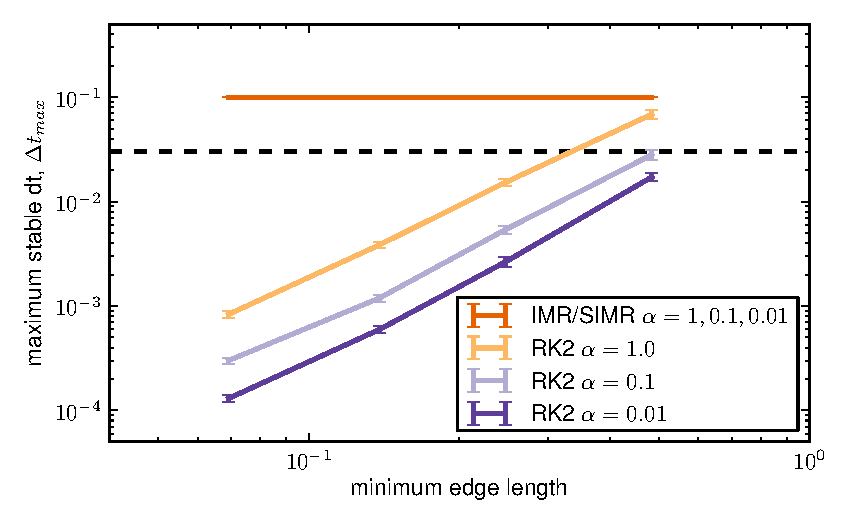
\includegraphics[width=\figsize]{images/stability_decoupled}
  \caption{Stable time step against discretisation size for LLG with FEM/BEM magnetostatics.}
  \label{fig:hms-stability}
\end{figure}


\begin{figure}[\figpos]
  \centering
  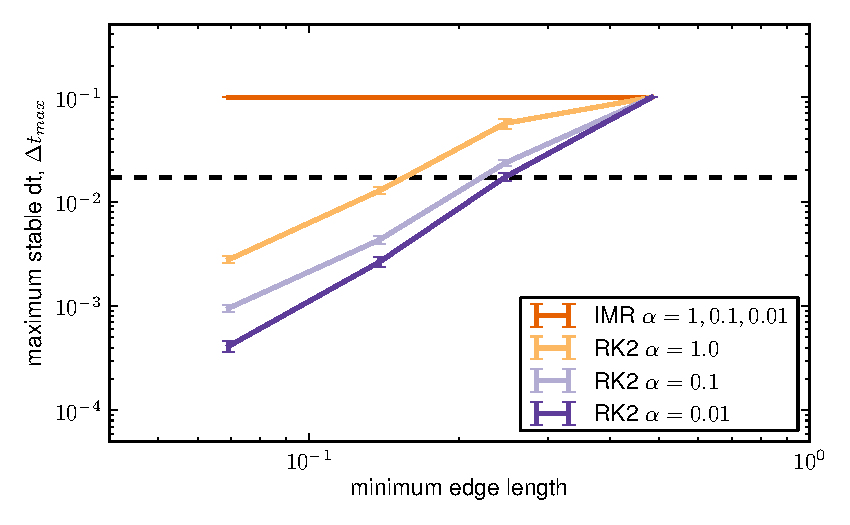
\includegraphics[width=\figsize]{images/stability_sphere}
  \caption{Stable time step against discretisation size for LLG with $\hv_{\text{ms}} = - \mv / 3$.
  }
  \label{fig:analytic-hms-stability}
\end{figure}

Comparing \autoref{fig:no-hms-stability} and \ref{fig:hms-stability} we see that using FEM/BEM magnetostatics significantly increases the stiffness, requiring roughly an order of magnitude smaller explicit time steps.
However, from \autoref{fig:analytic-hms-stability} we see that adding the exact field does not induce stiffness, so we can conclude that this effect is due to the FEM/BEM discretisation and not the magnetostatic field itself.
From our data we cannot predict whether other methods of calculating the magnetostatic field, such as multipole methods, will result in similar increases in the number of explicit time steps required.
However we expect that the effect is due to the coupling with the additional Poisson problems \iftransmagpaper\eqref{eq:fem-bem}\fi, thus any potential based method is likely to exhibit similar behaviour.

\autoref{fig:hms-stability} shows that using a semi-implicit method with explicit magnetostatic calculations (SIMR) imposes no stability restrictions on the time step due to spatial discretisation for the spatial resolutions required for micromagnetic problems.

To further analyse our results we need an estimate of the ratio of computational effort for explicit vs implicit time steps. Without magnetostatics we find that each step of IMR takes on average 5.86 times more computation time than a step of RK2. With magnetostatics each step of SIMR only takes 3.40 times more computation time than a step of RK2 (the difference is due to the cost of solving multiple Poisson problems at each Runge-Kutta stage). Using these ratios we can calculate the stable RK2 time step required to have equivalent computational efficiency to IMR with step size 0.1. This stable step size is marked on \autoref{fig:no-hms-stability}, \ref{fig:hms-stability} and \ref{fig:analytic-hms-stability} with a dashed line.

Based on these results we say that a problem is ``stiff'', and that an implicit method will perform significantly better than an explicit one, if the ratio of the desired time step, $\dtinitial$ to the maximum stable explicit time step, $\dtmax$ is greater than 20.
% This roughly agrees with the results of Suess \etal \cite{Suess2002}, who used the widely used (and presumably heavily optimised) CVODE package to solve the mumag standard problem 4 using similar techniques to ours. % Their bdf2 steps are extremely slow, probably bad preconditioner.
A caveat is that both types of model could be further optimised using, for example parallelism, improved preconditioning, mass lumping, boundary matrix compression\cite[Sec. 3]{Knittel2011} etc.

Typical advice for the number of elements per exchange length is that an absolute minimum number is one, and in order to show that the results are mesh independent the mesh must be refined a few times \cite[Sec. 11]{nmag-manual}.
This leads to a reasonable finest mesh with around three elements per exchange length.

We see that with FEM/BEM magnetostatics, realistic damping ($\alpha = 0.01$) and at least three elements per exchange length the problem is stiff.

Without FEM/BEM magnetostatics stiffness only occurs if refinement to around five or more elements per exchange length is needed for any part of the domain.
Problems that require this level of refinement include resolving the geometry in studies of granular or patterned media\cite{Suess2002} and resolving vortex-core-like structures\cite{Andreas2014}.

On the other hand LLG problems can be only moderately stiff if refinement is only needed up to the level of a few elements per exchange length, as is often required for simple geometries.
This is consistent with the fact that the mu-mag standard problem 4 is often solved using explicit integration methods with spatial refinement of around 0.5 exchange lengths \cite{mumag-website}.

Similar experiments with the standard 4th order Runge-Kutta method\cite[41]{Iserles2009} and $\alpha=1.0$ (plots not shown) give essentially the same results as for RK2. As $\alpha$ is reduced the maximum stable step size $\dtmax$ is reduced, but not as rapidly as for RK2. However due to the increased computational cost per time step (a factor of two) the onset of stiffness (for all $\alpha$) occurs at roughly the same spatial discretisation as for RK2 with $\alpha = 0.1$.

Finally we point out that the discussion above assumes that the accuracy obtained with $\dtx{} = \dtinitial$ is sufficient.
If higher accuracy than this is required then smaller time steps are needed regardless of stability, so the limitations imposed by stiffness are proportionally less significant.


\section{Conclusions}
Our results show that the LLG equation without magnetostatics or with analytical magnetostatic field calculations becomes stiff (\ie implicit methods are significantly more efficient) as the number of elements per exchange length decreases below around 5.
If FEM/BEM magnetostatic calculations are used stiffness occurs at much coarser discretisations, beginning at around $2\dash 3$ elements per exchange length.
In all cases decreasing the damping constant also increases the stiffness.

The results for the ODE version of the problem indicate that the observed stiffness is a result of the spatial discretisation and not the physics of the problem.
Since more complex physics is unlikely to reduce the stiffness, we expect that these results will extend to other, more complex, problems.

We also found that our semi-implicit FEM/BEM method does not suffer from discretisation induced stiffness.

\iftransmagpaper

\section*{Acknowledgement}
This project is funded by the Engineering and Physical Sciences Research Council (EPSRC) on grant number EP/G01705/1.

\bibliographystyle{IEEEtran}
\bibliography{IEEEabrv,small_bib}

\end{document}
\fi


%%% Local Variables:
%%% mode: latex
%%% TeX-master: t
%%% End:
